\documentclass
%[draft] %TODO rimuovere draft dopo aver localizzato overfull warning
{article}

\usepackage[italian]{babel}
\usepackage[utf8]{inputenc}


\usepackage{listings} % for coding like part

\usepackage{graphicx}
\graphicspath{ {./images/} }

% RELATIONAL DB SCHEMA
\usepackage{tikz}
\usetikzlibrary{shapes,positioning,calc}
\colorlet{lightgray}{gray!20}
% RELATIONAL DB SCHEMA


\usepackage{float} %#$@&*!

\usepackage{caption}
\usepackage{hyperref} % lasciare per ultimo
\hypersetup{colorlinks=true, linkcolor=blue, citecolor=black, plainpages=false, urlcolor=blue}

% huge indentation of paragraph only for demonstration purposes. 
%\setlength{\parindent}{5em} 
% some paragraph skip to better distinguish  lines of different paragraphs  
\setlength{\parskip}{.8em} 

\begin{document}
\begin{titlepage}
	\begin{center}
		\Huge{Progetto Basi di Dati}\\
		[20mm]
		\Large{Paolo Addis}\\
		\Large{Samuele Poz}\\
		\Large{Tristano Munini}\\
		[20mm]
		\Large{RENDERE CARINO}
	\end{center}
\end{titlepage}

\tableofcontents
\thispagestyle{empty}
\cleardoublepage
\setcounter{page}{1}

% REGOLE DI STILE
% - scrivere in modo impersonale no "abbiamo deciso di"
% - nelle immagini H o !ht ????
% NUOVO ATTENZIONE!!! TERAPIA-PRESCRITTA o TERAPIA_PRESCRITTA? Perché in fase Relazionale si usa _

% COSE DA RICORDARE
% NEI REQUISITI
% - aggiungere numero di accessi effettuati e numero di Pazienti, Ricovero, ecc
% - Evidenziare la necessità dell'ospedale di accedere spesso alle diagnosi di un dato paziente

%TODO -- FACOLTATIVO
% - NUOVO VINCOLO INTEGRITÀ:
%   - due ricoveri distinti di uno stesso paziente non possono avere intersezioni nei periodi [D.Inizio, D.Fine]


\section{Progettazione Concettuale}\label{sec:prog_conc}

\subsection{Raccolta ed Analisi dei Requisiti}

Si vuole modellare il seguente insieme di informazioni riguardanti un sistema
per la gestione delle diagnosi e delle terapie dei pazienti ricoverati in un
dato ospedale.
\begin{itemize}
	\item Di ogni ricovero, il sistema deve memorizzare il codice univoco, il
	      nome della divisione ospedaliera (Cardiologia, Reumatologia, Ortopedia,
	      \dots ), il paziente ricoverato, le date di inizio e fine del ricovero
	      e il motivo principale del ricovero.

	\item Di ogni paziente, il sistema deve memorizzare il codice sanitario
	      (univoco), il cognome, il nome, la data di nascita, il luogo di nascita
	      e la provincia di residenza. Per i pazienti residenti fuori regione,
	      vengono memorizzati anche il nome della ULSS e la regione di appartenenza.
	      Inoltre, per ogni paziente, è necessario memorizzare il totale delle
	      durate dei ricoveri.

	\item Di ogni diagnosi effettuata durante il ricovero del paziente, sono
	      memorizzati la patologia diagnosticata, col suo codice ICD10
	      (classificazione internazionale delle patologie) e l’indicazione della
	      sua gravità (grave: si/no), la data e il nome e cognome del medico che
	      ha effettuato la diagnosi.

	\item Nella base di dati si tiene traccia delle terapie prescritte ai pazienti
	      durante il ricovero. Di ogni terapia, si memorizzano il farmaco prescritto,
	      la dose giornaliera, le date di inizio e di fine della prescrizione, la
	      modalità di somministrazione ed il medico che ha prescritto la terapia.

	\item Di ogni farmaco sono memorizzati il nome commerciale (univoco), l’azienda
	      produttrice, il nome e la quantità dei principi attivi contenuti e la
	      dose giornaliera raccomandata.

	\item Si tiene, infine, traccia delle diagnosi che hanno motivato le terapie.
	      In particolare, ogni terapia è prescritta al fine di curare una o più
	      patologie diagnosticate. Può capitare anche che una nuova patologia
	      (registrata come nuova diagnosi) sia causata, come effetto collaterale,
	      da una terapia precedentemente prescritta. Tale legame causa-effetto va
	      registrato nella base di dati.
\end{itemize}
Tramite un portale web dovrà essere possibile accedere a tale base di dati ed
aggiungere o rimuovere pazienti, ricoveri, diagnosi con relative terapie e farmaci.
% TODO aggiungere esempio di Codice Ricovero (tipo RIC302) così poi nella fase logica si può dire Codice Diagnosi è stato creato ispirandosi a quello già presente (es RIC302DIA1), Codice Terapia es TER123
% TODO aggiungere numeri/necessità dell'ospedale 


\clearpage
\subsection{Progettazione del Modello E-R}

La progettazione dello schema Entità-Relazioni è avvenuto in tre fasi. 
Nella prima fase, la prima entità modellata è stata RICOVERO che memorizza tutte le informazioni relative a un ricovero e possiede come attributi: \textit{Codice Ricovero}, \textit{Divisione Ospedaliera}, \textit{Paziente Ricoverato}, \textit{Data Inizio}, \textit{Data Fine}, \textit{Motivo}. 
In particolare, l'attributo \textit{Codice Ricovero} è stato scelto come chiave primaria a causa della sua proprietà di unicità. 
Successivamente è stata modellata l'entità PAZIENTE che possiede i seguenti attributi: \textit{Codice Fiscale}, \textit{Cognome}, \textit{Nome}, \textit{Data di Nascita}, \textit{Luogo di Nascita} e \textit{Provincia di residenza} del paziente. L'attributo \textit{Codice Fiscale} è stato scelto come chiave primaria in quanto unico per ogni paziente.
Inoltre, è richiesto di memorizzare informazioni aggiuntive per i pazienti fuori regione. Per far ciò è stata creata una specializzazione PAZIENTE-FUORI-REGIONE di PAZIENTE i cui attributi sono: \textit{Regione di Appartenenza} e \textit{ULSS}. 
Nei requisiti sul paziente è richiesto, inoltre, di tener traccia del tempo totale trascorso all'interno dell'ospedale durante i ricoveri.
Quest'informazione è modellata attraverso \textit{Totale Giorni Ricoveri}, un attributo derivato su paziente che è la somma di tutte le durate dei ricoveri riguardanti il paziente.
La relazione di afferenza tra RICOVERO e PAZIENTE prende il nome VIENE-RICOVERATO.
L'informazione memorizzata nell'attributo \textit{Paziente Ricoverato} di RICOVERO viene salvata anche attraverso la nuova relazione, di conseguenza, per evitare ridondanze, è possibile rimuovere l'attributo dall'entità
% TODO magari nel testo e non come nota \footnote{Si ricorda che è preferibile evitare ridondanze perché inconsistenze bla bla }
.
Un nuovo paziente viene inserito nella base di dati la prima volta in cui viene ricoverato, di conseguenza la partecipazione di PAZIENTE alla relazione VIENE-RICOVERATO è totale.
Anche RICOVERO partecipa in modo totale alla relazione, in quanto sarebbe insensato inserire i dati di un ricovero senza specificare a chi si riferiscano.
Ogni paziente può essere ricoverato più volte ma ogni ricovero riguarda un solo paziente, dunque la relazione VIENE-RICOVERATO è della forma Uno-a-Molti.
\\
Successivamente è stata modellata l'entità DIAGNOSI che possiede come attributi: \textit{Data}, \textit{Medico} e \textit{Patologia}, un attributo composto formato da \textit{Codice} e \textit{Gravità}.
La chiave è composta dall'attributo \textit{Data} e dalla relazione EFFETTUATA-DURANTE.
Quest'ultima, del tipo Uno-a-Molti, lega l'entità RICOVERO a DIAGNOSI.
In particolare una diagnosi verrà inserita solo se nella base di dati è già presente il ricovero a cui afferisce, quindi la partecipazione di DIAGNOSI alla relazione è totale.
È importante introdurre un vincolo di integrità riguardante la data in cui viene effettuata la diagnosi in quanto deve essere compresa tra la data di inizio e quella di fine del ricovero.
Sarebbe perfettamente lecito, invece, avere un ricovero durante il quale non è stata effettuata alcuna diagnosi, questo stabilisce la partecipazione parziale di RICOVERO in EFFETTUATA-DURANTE.
Il Risultato della prima fase della progettazione è illustrata in \autoref{fig:paz-ric-dia}.

\begin{figure}[!ht] % TODO abbellire
  \centering
  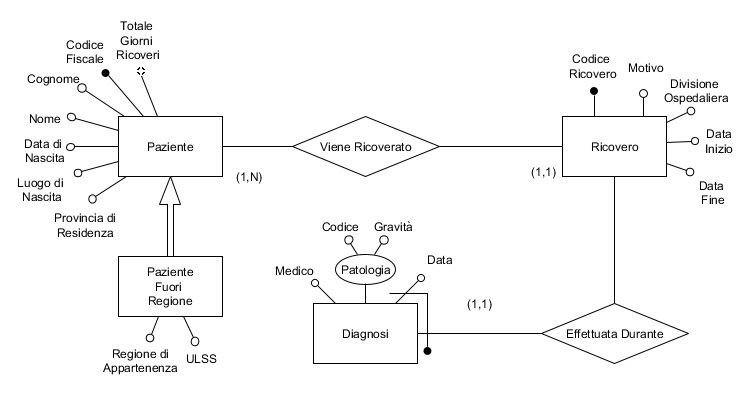
\includegraphics[width=\linewidth]{parte1}
  \caption{Prima parte}
	\label{fig:paz-ric-dia}
\end{figure}

La seconda fase considera il terzo ed il quarto punto dell'analisi dei requisiti in cui si chiede di tener traccia delle terapie e dei farmaci utilizzati.
Per questi ultimi è stata creata l'entità FARMACO con attributi: \textit{Dose Giornaliera Raccomandata}, \textit{Nome Commerciale}, \textit{Azienda Produttrice} e due attributi multivalore \textit{Nome Principi Attivi} e \textit{Quantità Principi Attivi}.
La chiave primaria è data dall'attributo \textit{Nome Commerciale} in quanto univoco.
Un farmaco può possedere uno o più principi attivi e deve necessariamente non esserne privo.
Per modellare l'entità TERAPIA si fa intuitivamente riferimento alla terapia come metodo astratto per curare più patologie, di conseguenza per quest'entità sono stati creati gli attributi: \textit{Dose Giornaliera} e \textit{Modalità Somministrazione}. Le richieste dei requisiti quali data di inizio e fine e medico prescrivente della terapia verrano trattate nella terza fase di progettazione. La chiave di TERAPIA è composta dagli attributi \textit{Dose Giornaliera} e \textit{Modalità Somministrazione} e dalla relazione SOMMINISTRATO-DURANTE che lega FARMACO a TERAPIA.
Questa relazione è della forma Uno-a-Molti in quanto in ogni terapia si somministra un solo farmaco mentre un farmaco può essere somministrato in più terapie. E' importate considerare il fatto che una terapia non può esistere senza un farmaco da somministrare, quindi la partecipazione di TERAPIA alla relazione SOMMINISTRATO-DURANTE è totale. D'altro canto un farmaco può essere memorizzato nella base di dati pur non essendo associato ad una particolare terapia, quindi la partecipazione di FARMACO alla precedente relazione è parziale. Questa seconda fase di progettazione è illustrata nella \autoref{fig:far-ter}

\begin{figure}[!ht] % TODO abbellire
  \centering
  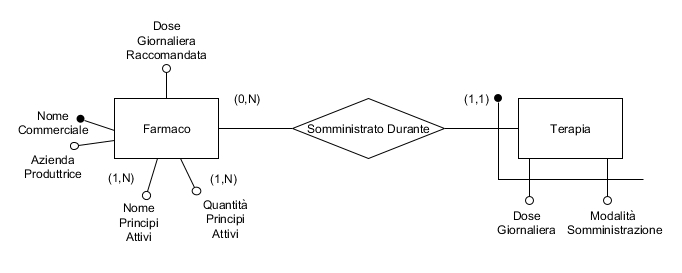
\includegraphics[width=\linewidth]{parte2}
  \caption{Seconda parte}
	\label{fig:far-ter}
\end{figure}

Nella terza fase della progettazione è stato modellato nello schema E-R l'ultimo punto dell'analisi dei requisiti attraverso la relazione MOTIVA-TERAPIA. Particolare attenzione è stata fatta alla parte in cui si specifica che una terapia può essere associata ad una diagnosi in due modi differenti: quello che la definisce come cura per una patologia e quello che la definisce come causa di una nuova patologia.  Va sottolineato che in entrambi i casi, nella base di dati, la patologia è salvata attraverso DIAGNOSI.

In un primo momento è stato modellato il sottoschema illustrato in \autoref{fig:piccolo1}.  Il modo in cui è stata definita l'entità TERAPIA permetterà di modellare il requisito \textit{ogni terapia può curare più patologie}.  Un'informazione come data di inizio, o data di fine, o medico prescrivente, non può essere memorizzata in TERAPIA perché, altrimenti, non sarebbe possibile applicare questa stessa terapia in uno spazio temporale differente, pena la perdita delle informazioni precedenti. D'altra parte non è nemmeno accettabile includere nella chiave primaria le informazioni relative alle date ed al medico, perché così facendo si differenzierebbero le entità, andando contro il requisito che si vuole modellare.  
Da qui la necessità di omettere attributi data inizio, data fine e medico prescrivente in TERAPIA, assegnandoli alla relazione MOTIVA-TERAPIA.  Intuitivamente questi attributi riguardano contemporaneamente la diagnosi, quindi la patologia che si vuole curare, e la terapia applicata, quindi il modo in cui si vuole affrontare la patologia, definendone il periodo in cui la terapia viene applicata e chi ha definito questo periodo.  
Nei requisiti è specificato che per alcune patologie manchino le cure, per questo motivo la partecipazione a MOTIVA-TERAPIA di DIAGNOSI è parziale.  Invece è sensato pensare che se una terapia esiste possa curare almeno una patologia, la partecipazione di TERAPIA quindi è totale.  
Nel complesso MOTIVA-TERAPIA, per ora, risulta essere una relazione Uno-A-Molti: nel testo è specificato che ad ogni diagnosi possa essere associata al più una terapia; mentre TERAPIA è stata definita appositamente per poter esser associata a più DIAGNOSI. 

\begin{figure}[!ht] % TODO abbellire
  \centering 
  \begin{minipage}{.5\textwidth}
    \centering
    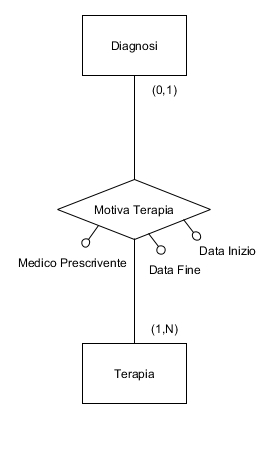
\includegraphics[width=\linewidth]{piccolo1}
    \caption{Prima modellazione}
    \label{fig:piccolo1}
  \end{minipage}%
  \begin{minipage}{.5\textwidth}
    \centering
    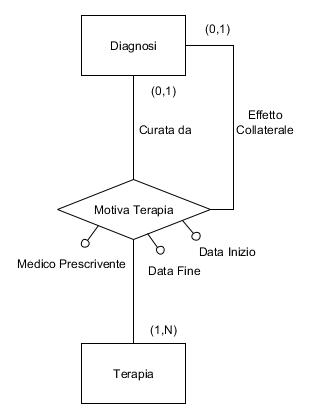
\includegraphics[width=\linewidth]{piccolo2}
    \caption{Relazione completa}
    \label{fig:piccolo2}
  \end{minipage}
\end{figure}

Successivamente è stato necessario modellare la situazione in cui una terapia prescritta è causa di una nuova patologia.  L'informazione che si vuole mantenere non dipende esclusivamente dall'entità TERAPIA ma dipende anche dal periodo di applicazione, quindi non è sufficiente creare una nuova relazione tra TERAPIA e DIAGNOSI, in quanto le informazioni aggiuntive sulla terapia sono memorizzate sulla relazione che le lega.  
La soluzione migliore è quella di trasformare MOTIVA-TERAPIA in una relazione ternaria: con DIAGNOSI che partecipa da una parte come patologia in cura e dall'altra come rilevazione di una nuova patologia.  
Per comodità, il risultato di tale trasformazione è riportato in \autoref{fig:piccolo2}.  
Ricordando che non tutte le applicazioni di una terapia causano un effetto collaterale e che ne possono causare al massimo uno, la partecipazione di DIAGNOSI come effetto collaterale è parziale con cardinalità 1. 

Al termine di questa terza fase di progettazione è necessario introdurre dei vincoli d'integrità per la relazione ternaria:
\begin{itemize}
  \item in ogni tripletta di MOTIVA-TERAPIA non può comparire due volte la     stessa DIAGNOSI;
  \item la DIAGNOSI che partecipa come effetto collaterale deve avere una data     successiva alla data della prima diagnosi.
\end{itemize}
%TODO ho dimenticato qualcosa?? 
Nella fase logica verrà mostrato che questa relazione può essere trasformata, senza perdita d'informazione, e con l'aggiunta di una nuova entità, in tre relazioni binarie. 

Dai requisiti è richiesto di memorizzare il medico che ha effettuato la diagnosi e il medico che ha prescritto la terapia. Ciò è stato fatto memorizzando le due informazioni attraverso l'introduzione dell'attributo \textit{Medico} in DIAGNOSI e \textit{Medico Prescrivente} in MOTIVA-TERAPIA. Non è stata introdotta un'entità rappresentativa del medico perchè scarna di informazione, di conseguenza il medico verrà rappresentato soltanto attraverso il proprio codice tramite gli attributi precedentemente specificati. 
% TODO Medico?
In conclusione lo schema Entità-Relazioni si presenta come in \autoref{fig:ER_progettazione_modello}.

\begin{figure}[H] % TODO abbellire
    \centering
    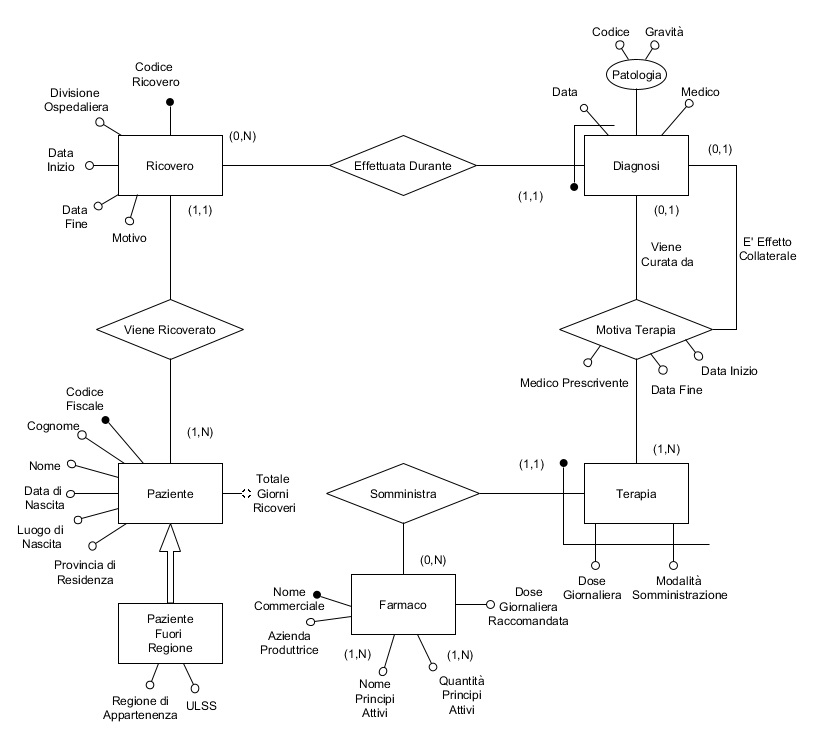
\includegraphics[width=\linewidth]{schema1}
    \caption{Lo schema Entità-Relazioni completo}
    \label{fig:ER_progettazione_modello}
\end{figure}


%\begin{figure}[h] % TODO abbellire
%\caption{Entità PAZIENTE con specializzazione e, a destra, RICOVERO}
%
\includegraphics[width=0.4\textwidth]{galaxy}
%
\includegraphics[width=0.4\textwidth]{galaxy}
%\end{figure}




\clearpage
\section{Progettazione Logica}

%TODO
%Cose che si potrebbero aggiungere:
% - Partizionamento di una relazione (si può fare con MEDICO collegato a PAZIENTE e DIAGNOSI)
%   (secondo Tri 'fare solo se non abbiamo abbastanza materiale')

\subsection{Ristrutturazione del Modello E-R}
\subsubsection{Semplificazione dei Concetti}
%% logical design steps
% ristrutturazione semplificare ER
% schema ristrutturato
% ottimizzazione analisi ridondanze
% schema con ridondanza
% elenco tabelle
% vincoli d'integrità

È utile semplificare strutture come specializzazioni, attributi composti e attributi multivalore perché renderà più facile la traduzione del modello Entità-Relazioni in quello Relazionale.

Ricordando che quest'ultimo non permette di rappresentare generalizzazioni sarà necessario rimuovere tutte le specializzazioni dal nostro schema E-R.
Si può notare che la specializzazione PAZIENTE-FUORI-REGIONE può essere facilmente rappresentata aggiungendo due attributi all'entità PAZIENTE.
I nuovi attributi, \textit{ULSS} e \textit{Regione di Appartenenza}, in PAZIENTE saranno facoltativi poiché la specializzazione è parziale.
La rimozione delle generalizzazioni non è sempre così immediata: se PAZIENTE-FUORI-REGIONE avesse avuto una relazione in più rispetto al genitore si sarebbero dovute valutare varie opzioni.
Per esempio la creazione di una nuova relazione per simboleggiare il legame tra genitore e figlio, lasciando invariati gli attributi.
Oppure la duplicazione nel figlio di tutti gli attributi e di tutte le relazioni del genitore.

Anche nel caso degli attributi composti la semplificazione è intuitiva, infatti nello schema l'unico attributo composto è \textit{Patologia} in DIAGNOSI.
Può essere trasformato in due nuovi attributi \textit{Codice Patologia} e \textit{Gravità Patologia} che contengono esattamente la stessa informazione.

Bisogna prestare più attenzione agli attributi multivalore:
in FARMACO sono presenti \textit{Nome Principi Attivi} e \textit{Quantità Principi Attivi} entrambi obbligatori e multivalore.
L'unica semplificazione attuabile è creare una nuova entità chiamata PRINCIPIO-ATTIVO è metterla in relazione Molti-A-Molti con FARMACO attraverso la nuova relazione CONTIENE.
PRINCIPIO-ATTIVO avrà un solo attributo, scelto anche come chiave primaria, chiamato \textit{Nome}, mentre alla relazione CONTIENE verrà aggiunto l'attributo \textit{Quantità}.
In questo modo saranno modellate esattamente le stesse informazioni precedentemente modellate dagli attributi multivalore.
% TODO in realtà ora le informazioni sono "sicure" nel senso che prima l'ordine in cui si inserivano nomi e quantità modificavano la reale informazione

\begin{figure}[!ht] % TODO abbellire
  \centering
  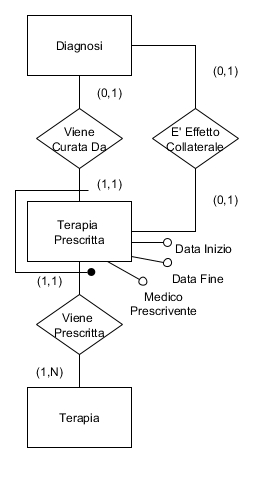
\includegraphics[width=.4\linewidth]{piccolo3}
  \caption{Il risultato della trasformazione di MOTIVA-TERAPIA}
  \label{fig:piccolo3}
\end{figure}

Un'ulteriore trasformazione da effettuare riguarda la relazione ternaria.
Infatti MOTIVA-TERAPIA, come è stato accennato in precedenza%TODO verificare accennamento
, può essere espressa tramite relazioni binarie.
In Figura \autoref{fig:piccolo3} si può vedere il risultato di tale trasformazione.
Si nota subito la nuova entità TERAPIA-PRESCRITTA, creata proprio per rappresentare una particolare applicazione di una terapia al fine di curare una patologia di una specifica diagnosi.
La nuova entità, quindi, è caratterizzata da:
\textit{Data Inizio} che indica il giorno in cui il paziente dovrà iniziare la terapia;
\textit{Data Fine} che indica il giorno in cui il paziente terminerà la terapia;
\textit{Medico Prescrivente} che indica il medico che ha prescritto la terapia e deciso il periodo di applicazione.
Osservando che la relazione MOTIVA-TERAPIA non può esistere senza la partecipazione simultanea di DIAGNOSI (come \textit{Viene Curata da}) e di TERAPIA si è deciso di rendere TERAPIA-PRESCRITTA un'entità debole.
La chiave primaria è composta dalle nuove relazioni binare VIENE-CURATA-DA e VIENE-PRESCRITTA, per entrambe la partecipazione di TERAPIA-PRESCRITTA è totale, mentre la cardinalità è al massimo uno. %TODO cardinalità 1 suona male
DIAGNOSI e TERAPIA interagiscono con le nuove relazioni, rispettivamente, nello stesso modo con cui interagivano con la relazione ternaria.
Per quanto riguarda \textit{È Effetto Collaterale} si può dire che rappresenti perfettamente la possibilità che una terapia prescritta possa causare una nuova patologia.
Notare che le partecipazioni sono appunto parziali.
Ovviamente anche il vincolo d'integrità precedentemente definito, dovrà essere modificato:
\begin{itemize}
  \item TERAPIA-PRESCRITTA non può essere in relazione \textit{È Effetto Collaterale} con la DIAGNOSI con cui definisce la sua chiave primaria;
  \item TERAPIA-PRESCRITTA non può essere in relazione \textit{È Effetto Collaterale} con una DIAGNOSI che ha una data successiva alla data della DIAGNOSI con cui definisce la sua chiave primaria; % TODO data precedente?
\end{itemize}
A questo punto, osservando nuovamente i sottoschemi in Figura \autoref{fig:piccolo2} ed in Figura \autoref{fig:piccolo3}, è chiaro che modellino ogni possibile situazione:
\begin{itemize}
  \item una DIAGNOSI a cui non è ancora stata assegnata una terapia;
  \item la prescrizione di una specifica terapia;
  \item la scoperta di una nuova patologia, attraverso una nuova diagnosi, causata dall'applicazione di una terapia;
  \item la possibilità che una TERAPIA possa curare più patologie (registrate attraverso DIAGNOSI differenti).
%TODO ci sono tutte?
\end{itemize}

Durante la fase di semplificazione dei concetti vengono analizzate anche le chiavi primarie delle entità.
Quando una chiave è troppo complessa, cioè composta da molti elementi, è bene sostituirla, così facendo si faciliteranno tutte le operazioni sulla base di dati.
Si ricorda che un'entità può disporre di chiavi candidate, cioè insiemi di attributi che, per loro natura, rispettano la proprietà di chiave primaria ma che, per qualche motivo, non sono stati scelti come tale.
Ora è naturale verificare se tra queste chiavi opzionali ce n'è una che, dopo tutte le semplificazioni effettuate allo schema E-R, è migliore della chiave primaria.
Purtroppo questa soluzione non è sempre possibile, infatti non è raro che le entità siano tra loro distinguibili soltanto per mezzo di un preciso insieme di attributi.
Nello schema E-R considerato fino ad ora non sono presenti chiavi candidate migliori delle chiavi primarie attuali, infatti la chiave primaria della maggior parte delle entità è composta da un solo attributo.

Rimangono da analizzare DIAGNOSI, TERAPIA e la nuova TERAPIA-PRESCRITTA.
La chiave primaria di quest'ultima, per il modo in cui l'entità è stata costruita, non può essere modificata a meno di introdurre pesanti vincoli di integrità.
Ora sorge un problema: TERAPIA-PRESCRITTA è un'entità debole che dipende da due entità a loro volta deboli.
Ciò significa che per identificare una terapia prescritta si deve risalire al ricovero da una parte ed al farmaco dall'altra, nel mentre si deve anche ricordare \textit{Data} in DIAGNOSI, \textit{Dose Giornaliera} e \textit{Modalità Somministrazione} in TERAPIA.
Intuitivamente questo equivale ad avere una chiave primaria in TERAPIA-PRESCRITTA composta da 5 elementi.
Quindi si propone di creare sia in DIAGNOSI che in TERAPIA un nuovo attributo chiamato, rispettivamente, \textit{Codice Diagnosi} e \textit{Codice Terapia} che conterrà un valore alfa numerico simile a quello contenuto in \textit{Codice Ricovero}.
%TODO servono vincoli integrità nuovi? Non mi pare

Applicando tutte le semplificazioni sopra descritte si ottiene lo schema E-R illustrato In \autoref{fig:ER_ristrutturato}.

\begin{figure}[H] % TODO abbellire
	\centering
	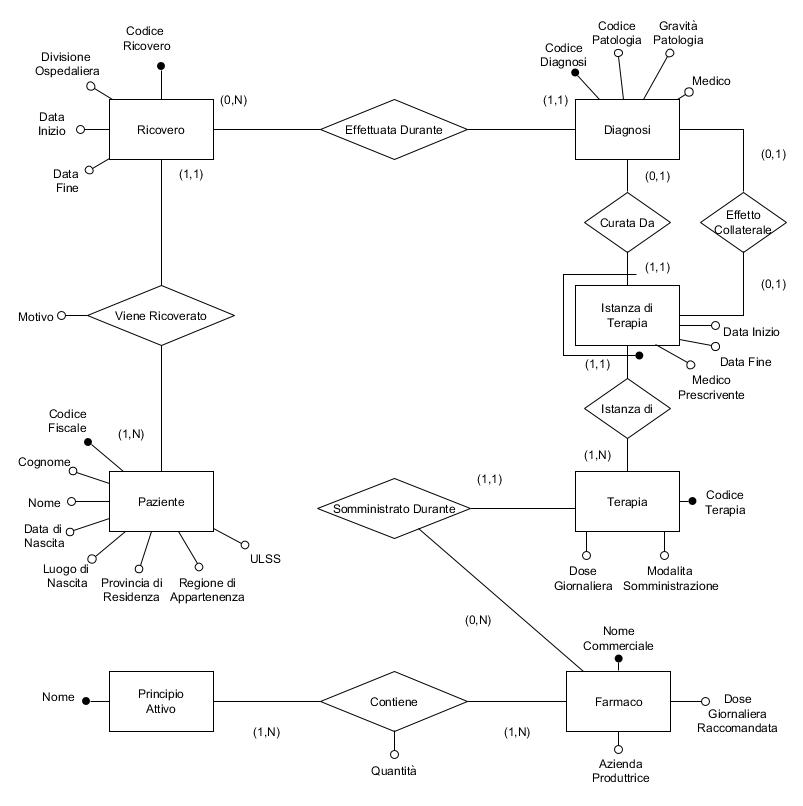
\includegraphics[width=\linewidth]{schema2}
	\caption{Lo schema Entità-Relazioni completo}
  \label{fig:ER_ristrutturato}
\end{figure}

\clearpage


% TODO NELLA FASE LOGICA
% - verrà aggiunta relazione tra PAZIENTE DIAGNOSI (es EFFETTUATA A) per verificare la differenza di prestazioni
% - l'unica ridondanza è data da EFFETTUATA A, la ricorsione DIAGNOSI->DIAGNOSI (o ISTANZA DI TERAPIA -> DIAGNOSI) NON è ridondanza (esprime informazioni differenti)

\subsubsection{Analisi delle Ridondanze}

Ai fini di ottimizzare le prestazioni, è stato studiato se risultasse conveniente mantenere l'attributo derivato \textit{Totale Giorni Ricoveri} dell'entità PAZIENTE.

\begin{figure}[H] % TODO abbellire
	\centering
	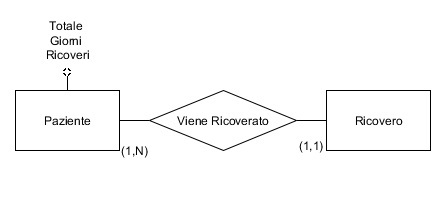
\includegraphics[width=\linewidth]{totalegiorni}
	\caption{Attributo derivato Totale Giorni Ricoveri}
	\label{fig:attributo-ridondante}
\end{figure}

I volumi stimati sono riportati in \autoref{tab:volumi-attributo-ridondante} e la frequenza delle operazioni interessate in \autoref{tab:operazioni-attributo-ridondante}.
% TODO aggiungere operazione di modifica date dei ricoveri

\begin{table}[H]
	\centering
	\begin{tabular}{|l|c|r|}
		\hline
		\textbf{Concept} & \textbf{Type} & \textbf{Volume} \\ \hline
		Paziente         & E             & 100000          \\ \hline
		Ricovero         & E             & 300000          \\ \hline
		Viene Ricoverato & R             & 300000          \\ \hline
	\end{tabular}
	\caption{Tabella dei volumi ridotta}
	\label{tab:volumi-attributo-ridondante}
\end{table}

\begin{table}[H]
	\centering
	\begin{tabular}{|l|c|r|}
		\hline
		\textbf{Operation}                  & \textbf{Type} & \textbf{Frequency} \\ \hline
		Registrazione Ricovero              & I             & 175/giorno         \\ \hline
		Controllo totale giorni di ricoveri & I             & 175/giorno         \\ \hline %TODO fix questo numero
	\end{tabular}
	\caption{Tabella delle operazioni ridotta}
	\label{tab:operazioni-attributo-ridondante}
\end{table}

In presenza dell'attributo derivato, per l'operazione di registrazione di un nuovo ricovero è necessario 1 accesso in scrittura per l'entità RICOVERO, 1 accesso in scrittura per la relazione VIENE-RICOVERATO, 1 accesso in lettura e 1 accesso in scrittura per l'entità PAZIENTE per leggere e aggiornare l'attributo \textit{Totale Giorni Ricoveri}.
Per l'operazione di verifica del totale dei giorni di ricoveri è sufficiente 1 accesso in lettura all'entità PAZIENTE.

\begin{table}[H]
	\centering
	\begin{tabular}{|l|c|c|c|}
		\hline
		\textbf{Concept} & \textbf{Type} & \textbf{Access} & \textbf{Type} \\ \hline
		\multicolumn{4}{|c|}{Registrazione Ricovero}                       \\ \hline
		Ricovero         & E             & 1               & W             \\ \hline
		Viene Ricoverato & R             & 1               & W             \\ \hline
		Paziente         & E             & 1               & R             \\ \hline
		Paziente         & E             & 1               & W             \\ \hline
		\multicolumn{4}{|c|}{Controllo totale giorni di ricoveri}          \\ \hline
		Paziente         & E             & 1               & R             \\ \hline
	\end{tabular}
	\caption{Tabella dei costi, caso con ridondanza}
	\label{tab:costi-attributo-ridondante}
\end{table}

Considerando il costo di 1 accesso in scrittura come 2 accessi in lettura, calcoliamo il numero di accessi complessivo giornaliero per le 2 operazioni nel caso con ridondanza:
\begin{equation}
	(3W + 1R) \times 175 + 1R \times 175 \approx 1400R
\end{equation}

Rimuovendo l'attributo, per l'operazione di registrazione di un nuovo ricovero è sufficiente 1 accesso in scrittura per l'entità RICOVERO e 1 accesso in scrittura per la relazione VIENE-RICOVERATO.
Per l'operazione di verifica del totale dei giorni di ricoveri, considerando la tabella dei volumi, sono necessari in media 3 accessi in lettura per la relazione VIENE-RICOVERATO e 3 accessi in lettura per l'entità RICOVERO.

\begin{table}[H]
	\centering
	\begin{tabular}{|l|c|c|c|}
		\hline
		\textbf{Concept} & \textbf{Type} & \textbf{Access} & \textbf{Type} \\ \hline
		\multicolumn{4}{|c|}{Inserimento Diagnosi}                         \\ \hline
		Viene Ricoverato & R             & 1               & W             \\ \hline
		Ricovero         & R             & 1               & W             \\ \hline
		\multicolumn{4}{|c|}{Stampa Storico Diagnosi}                      \\ \hline
		Viene Ricoverato & R             & 3               & R             \\ \hline
		Ricovero         & E             & 3               & R             \\ \hline
	\end{tabular}
	\caption{Tabella dei costi, caso senza ridondanza}
	\label{tab:costi-no-attributo-ridondante}
\end{table}

Considerando il costo di 1 accesso in scrittura come 2 accessi in lettura, calcoliamo il numero di accessi complessivo giornaliero per le 2 operazioni nel caso senza ridondanza:
\begin{equation}
	2W \times 175 + 6R \times 175 \approx 1750R
\end{equation}

Risulta conveniente mantenere l'attributo \textit{Totale Giorni Ricoveri}.

Lo schema Entità-Relazioni in \autoref{fig:ER_ristrutturato} non presenta ulteriori ridondanze, infatti, il ciclo DIAGNOSI TERAPIA-PRESCRITTA DIAGNOSI non è ridondante. Tuttavia visto il requisito di stampa delle diagnosi effettuate da un singolo paziente consideriamo l'inserimento della relazione:
\begin{itemize}
	\item EFFETTUATA A: una relazione Uno-A-Molti tra PAZIENTE
	      e DIAGNOSI. La partecipazione di PAZIENTE è parziale mentre quella
	      di DIAGNOSI è totale.
\end{itemize}

Viene creato quindi il ciclo in \autoref{fig:ciclo-ridondanza} PAZIENTE, RICOVERO, DIAGNOSI dato dalle relazioni VIENE RICOVERATO, EFFETTUATA DURANTE, EFFETTUATA A.

\begin{figure}[H] % TODO abbellire
	\centering
	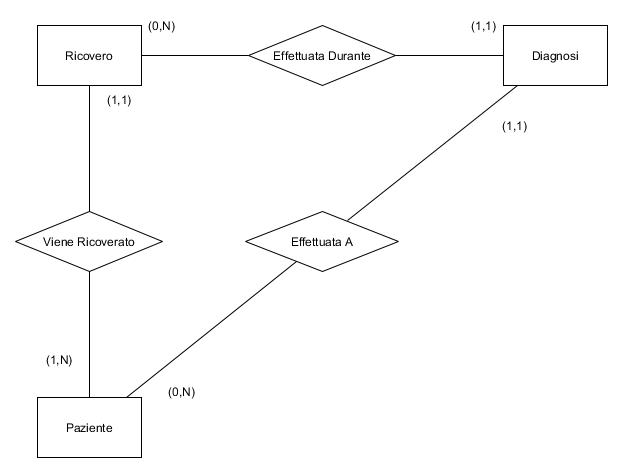
\includegraphics[width=\linewidth]{schema3}
	\caption{Ciclo con ridondanza}
	\label{fig:ciclo-ridondanza}
\end{figure}
Si procede con il valutare se è conveniente mantenere la relazione EFFETTUATA A tra PAZIENTE e DIAGNOSI in funzione della frequenza delle operazioni di inserimento nuove diagnosi e stampa dello storico diagnosi di un paziente.

% TODO REQUISITO specificare nei requisiti le operazioni richieste e i volumi

I volumi stimati sono riportati in \autoref{tab:volumi-ciclo} e la frequenza delle operazioni interessate in \autoref{tab:operazioni-ciclo}

% TODO REQUISITO spostare table:volumi nei requisiti, no non si può non tutti esistono nei requisiti
\begin{table}[H]
	\centering
	\begin{tabular}{|l|c|r|}
		\hline
		\textbf{Concept}      & \textbf{Type} & \textbf{Volume} \\ \hline
		Paziente              & E             & 100000          \\ \hline
		Ricovero              & E             & 300000          \\ \hline
		Diagnosi              & E             & 1200000         \\ \hline
		Terapia               & E             & 30000           \\ \hline
		Istanza di Terapia    & E             & 1200000         \\ \hline
		Farmaco               & E             & 10000           \\ \hline
		Viene Ricoverato      & R             & 300000          \\ \hline
		Effettuata Durante    & R             & 1200000         \\ \hline
		Effettuta A           & R             & 1200000         \\ \hline
		Curata Da             & R             & 1200000         \\ \hline
		Istanza Di            & R             & 1200000         \\ \hline
		Effetto Collaterale   & R             & 50000           \\ \hline
		Somministrato Durante & R             & 10000           \\ \hline
	\end{tabular}
	\caption{Tabella dei volumi}
	\label{tab:volumi}
\end{table}

\begin{table}[H]
	\centering
	\begin{tabular}{|l|c|r|}
		\hline
		\textbf{Concept}   & \textbf{Type} & \textbf{Volume} \\ \hline
		Paziente           & E             & 100000          \\ \hline
		Ricovero           & E             & 300000          \\ \hline
		Diagnosi           & E             & 1200000         \\ \hline
		Viene Ricoverato   & R             & 300000          \\ \hline
		Effettuata Durante & R             & 1200000         \\ \hline
		Effettuata A       & R             & 1200000         \\ \hline
	\end{tabular}
	\caption{Tabella dei volumi ridotta}
	\label{tab:volumi-ciclo}
\end{table}

\begin{table}[H]
	\centering
	\begin{tabular}{|l|c|r|}
		\hline
		\textbf{Operation}      & \textbf{Type} & \textbf{Frequency} \\ \hline
		Inserimento Diagnosi    & I             & 700/giorno         \\ \hline
		Stampa Storico Diagnosi & I             & 1400/giorno        \\ \hline
	\end{tabular}
	\caption{Tabella delle operazioni ridotta}
	\label{tab:operazioni-ciclo}
\end{table}

Nel caso con ridondanza per l'operazione di inserimento di una nuova diagnosi sono necessari 1 accesso in scrittura per l'entità DIAGNOSI e 1 accesso in scrittura per entrambe le relazioni EFFETTUATA DURANTE e EFFETTUATA A.
Per l'operazione di stampa delle diagnosi di un paziente sono necessari 12 accessi in lettura per la relazione EFFETTUATA A e 12 accessi in lettura per l'entità DIAGNOSI.

Considerando il costo di 1 accesso in scrittura come 2 accessi in lettura, calcoliamo il numero di accessi complessivo giornaliero per le 2 operazioni nel caso con ridondanza:
\begin{equation}
	3W \times 700 + 24R \times 1400 \approx	37800R
\end{equation}

\begin{table}[H]
	\label{table:3}
	\centering
	\begin{tabular}{|l|c|c|c|}
		\hline
		\textbf{Concept}    & \textbf{Type} & \textbf{Access} & \textbf{Type} \\ \hline
		\multicolumn{4}{|c|}{Inserimento Diagnosi}                            \\ \hline
		Diagnosi            & E             & 1               & W             \\ \hline
		Effettutata Durante & R             & 1               & W             \\ \hline
		Effettuata A        & R             & 1               & W             \\ \hline
		\multicolumn{4}{|c|}{Stampa Storico Diagnosi}                         \\ \hline
		Effettuata A        & R             & 12              & R             \\ \hline
		Diagnosi            & E             & 12              & R             \\ \hline
	\end{tabular}
	\caption{Tabella dei costi, caso con ridondanza}
\end{table}

Nel caso senza ridondanza per l'operazione di inserimento di una nuova diagnosi sono necessari 1 accesso in scrittura per l'entità DIAGNOSI e 1 accesso in scrittura per la relazione EFFETTUATA DURANTE.
Per l'operazione di stampa delle diagnosi di un paziente sono necessari 3 accessi in lettura per la relazione VIENE RICOVERATO, 12 accessi in lettura per la relazione EFFETTUATA DURANTE e 12 accessi in lettura per l'entità DIAGNOSI.

Considerando il costo di 1 accesso in scrittura come 2 accessi in lettura, calcoliamo il numero di accessi complessivo giornaliero per le 2 operazioni nel caso senza ridondanza:
\begin{equation}
	2W \times 700 + 27R \times 1400 \approx	40600R
\end{equation}

\begin{table}[H]
	\label{table:4}
	\centering
	\begin{tabular}{|l|c|c|c|}
		\hline
		\textbf{Concept}    & \textbf{Type} & \textbf{Access} & \textbf{Type} \\ \hline
		\multicolumn{4}{|c|}{Inserimento Diagnosi}                            \\ \hline
		Diagnosi            & E             & 1               & W             \\ \hline
		Effettutata Durante & R             & 1               & W             \\ \hline
		\multicolumn{4}{|c|}{Stampa Storico Diagnosi}                         \\ \hline
		Viene Ricoverato    & R             & 3               & R             \\ \hline
		Effettutata Durante & R             & 12              & R             \\ \hline
		Diagnosi            & E             & 12              & R             \\ \hline
	\end{tabular}
	\caption{Tabella dei costi, caso senza ridondanza}
\end{table}

Concludiamo che è conveniente mantenere la ridondanza visto il costo minore delle operazioni giornaliere.

\begin{figure}[!ht] % TODO abbellire
    \centering
    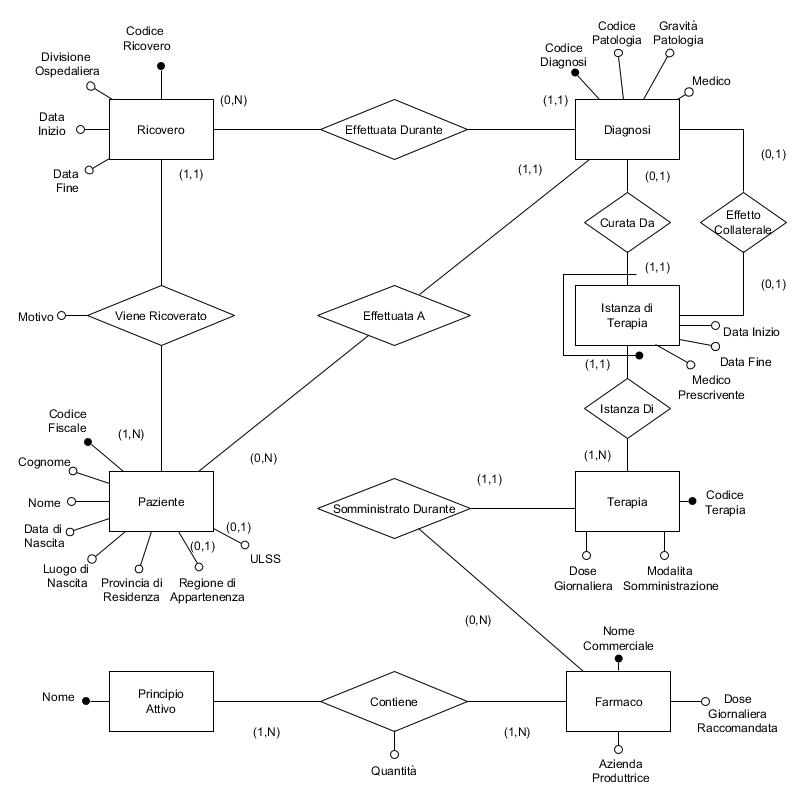
\includegraphics[width=\linewidth]{schema4}
    \caption{Lo schema Entità-Relazioni finale}
    \label{fig:ER_finale}
\end{figure}



\clearpage
\subsection{Traduzione da ER a Relazionale}

% TODO leggere capitolo 14 Elmasri
% TODO leggere capitolo 9 Atzeni

In questa fase della progettazione logica è possibile iniziare la traduzione del modello E-R in quello Relazionale.
Come prima cosa, in quanto immediato, ogni entità verrà rappresentata sotto forma di tupla. %TODO verifica correttezza 
Queste tuple verranno poi modificate per poter mantenere anche le informazioni relative alle relazioni, può capitare che ad una relazione venga associata un nuova tupla.
%TODO idea generale di modello relazionale Le tuple saranno raccolte in varie tabelle in cui ogni riga

In (fig relazionale-iniziale) %TODO FIX \autoref{fig:relazionale_iniziale}
si può vedere una prima modellazione dello schema Relazionale, con le seguenti tuple:
\begin{itemize} % TODO abbellire
  \item PAZIENTE(\textit{\underline{Codice\_Fiscale}, Cognome, Nome, Data\_di\_Nascita,\\
    Luogo\_di\_Nascita, Provincia\_di\_Residenza, Regione\_di\_Appartenenza,\\
  ULSS, Totale\_Giorni\_Ricovero}) con \textit{Codice\_Fiscale} come chiave primaria.
  Per motivi di spazio, rappresentata nello schema in una forma compatta;
  \item RICOVERO(\textit{\underline{Codice\_Ricovero}, Data\_Inizio, Data\_Fine, Motivo,\\Divisione\_Ospedaliera}) con \textit{Codice\_Ricovero} come chiave primaria;
  \item DIAGNOSI(\textit{\underline{Codice\_Diagnosi}, Data, Codice\_Patologia, Gravità\_Patologia,\\Medico}) con \textit{Codice\_Diagnosi} come chiave primaria;
  \item TERAPIA(\textit{\underline{Codice\_Terapia}, Dose\_Giornaliera,\\Modalità\_Somministrazione}) con \textit{Codice\_Terapia} come chiave primaria;
  \item FARMACO(\textit{\underline{Nome\_Commerciale}, Dose\_Giornaliera\_Raccomandata,\\Azienda\_Produttrice}) con \textit{Nome\_Commerciale} come chiave primaria;
  \item PRINCIPIO\_ATTIVO(\textit{\underline{Nome}}) con \textit{Nome} come chiave primaria. 
\end{itemize}
% TODO sistemare sta cavolo di larghezza... Causa: latex non sa spaccare PAROLA_PAROLA
Bisogna prestare più attenzione a TERAPIA\_PRESCRITTA perché, in quanto entità debole, la sua chiave primaria dipende dalle relazioni\\VIENE\_CURATA\_DA e VIENE\_PRESCRITTA, o meglio, comprende degli\\identificatori esterni.
Nel dettaglio un identificatore sarà dato dalla chiave primaria di DIAGNOSI mentre l'altro dalla chiave primaria di TERAPIA.
Si ricorda che le entità identificate esternamente partecipano alle associazioni identificanti sempre con una cardinalità minima e massima pari a uno.
Quindi, nonostante le due relazioni siano di tipi differenti (Uno-A-Uno ed Uno-A-Molti), possono essere trattate allo stesso modo, cioè aggiungendo alla tupla
\vspace{3mm}
\\
\hspace{10mm}
TERAPIA\_PRESCRITTA(\textit{Data\_Inizio, Data\_Fine, Medico\_Prescrivente})
\vspace{3mm}
\\
i nuovi valori referenziali \textit{Diagnosi} e \textit{Terapia}.
Questi, rispettivamente, conterranno il valore \textit{Codice\_Diagnosi} e \textit{Codice\_Terapia} delle tuple dalle quali TERAPIA\_PRESCRITTA dipende.
La tupla risultante è la seguente:
\vspace{3mm}
\\ TERAPIA\_PRESCRITTA(\textit{\underline{Codice\_Diagnosi}, \underline{Codice\_Terapia}, Data\_Inizio, Data\_Fine, Medico\_Prescrivente})
\vspace{3mm}
\\
la chiave primaria è composta dalla coppia (\textit{Codice\_Diagnosi, Codice\_Terapia}).

In questi passaggi, in realtà, è stato fatto qualcosa di più di una semplice traduzione di una entità dal modello E-R a quello Relazione, infatti sono state tradotte anche due relazioni.

La prima è VIENE\_CURATA\_DA che fornisce l'informazione: una patologia, trovata per mezzo di una diagnosi, può essere curata con l'applicazione di una particolare terapia.
Quest'informazione, nel modello relazionale, può essere trovata cercando, tra tutte le tuple per le terapie prescritte, una che abbia il campo \textit{Diagnosi} uguale al campo \textit{Codice\_Diagnosi}.
Notare che non esiste nessuna certezza che tale tupla esista.
Questa possibilità è consistente con quanto modellato nello schema E-R (la partecipazione di DIAGNOSI è parziale).
Bisogna, invece, introdurre un vincolo che vieti che due tuple del tipo TERAPIA\_PRESCRITTA referenzino la stessa diagnosi, in altre parole bisogna assicurare la proprietà di chiave al campo \textit{Diagnosi}.

\begin{tikzpicture} % TODO spostare dopo la spiegazione
  [relation/.style={
    rectangle split,
    rectangle split parts=#1,
    rectangle split part align=base,
    draw,
    anchor=center,
    align=center,
    text height=3mm,
    text centered
    }
  ]
  %\hspace*{-0.2cm} % tutto un po' più a  sinistra

  % RELATIONS
  
  % TODO FIX
  %\node (pazientetitle) {\textbf{PAZIENTE}};
  %\node [
  %  relation=6,
  %  rectangle split horizontal,
  %  rectangle split part fill={lightgray!50},
  %  anchor=north west,
  %  below=0.6cm of pazientetitle.west,
  %  anchor=west
  %  ]
  %  (paziente1)
  %  {
  %   \underline{Codice\_Fiscale}%
  %   \nodepart{two}   Cognome
  %   \nodepart{three} Nome
  %   \nodepart{four}  Data\_di\_Nascita
  %   \nodepart{five}  Luogo\_di\_Nascita
  %  };
  %\node [
  %  relation=5,
  %  rectangle split horizontal,
  %  rectangle split part fill={lightgray!50},
  %  anchor=north west,
  %  below=1.1cm of paziente1.west,
  %  anchor=west
  %  ]
  %  (paziente2)
  %  {
  %   \nodepart[dashed]{one}
  %   \nodepart{two}  Provincia\_\\di\_\\Residenza
  %   \nodepart{three}  Regione\_\\di\_\\Appartenenza
  %   \nodepart{four}  ULSS
  %   \nodepart{five}  Totale\_\\Giorni\_\\Ricoveri
  %  };
  % TODO END FIX
  
  
  \node (pazientetitle) {\textbf{PAZIENTE}};
  \node [
    relation=5,
    rectangle split horizontal,
    rectangle split part fill={lightgray!50},
    anchor=north west,
    below=0.6cm of pazientetitle.west,
    anchor=west
    ]
    (paziente)
    {
     \underline{Codice\_Fiscale}%
     \nodepart{two}   Cognome
     \nodepart{three} Nome
     \nodepart{four} \dots
     \nodepart{five} Luogo\_di\_Nascita
    };
  
  \node [below=1.3cm of paziente.west, anchor=west] (ricoverotitle) {\textbf{RICOVERO}};
  \node [
    relation=5,
    rectangle split horizontal,
    rectangle split part fill={lightgray!50},
    anchor=north west,
    below=0.6cm of ricoverotitle.west,
    anchor=west
    ]
    (ricovero)
    {
     \underline{Codice\_Ricovero}%
     \nodepart{two}   Data\_Inizio
     \nodepart{three} Data\_Fine
     \nodepart{four}  Motivo
     \nodepart{five}  Divisione\_Ospedaliera
    };
  
  \node [below=1.3cm of ricovero.west, anchor=west] (diagnosititle) {\textbf{DIAGNOSI}};
  \node [
    relation=5,
    rectangle split horizontal,
    rectangle split part fill={lightgray!50},
    anchor=north west,
    below=0.6cm of diagnosititle.west,
    anchor=west
    ]
    (diagnosi)
    {
     \underline{Codice\_Diagnosi}%
     \nodepart{two}   Data
     \nodepart{three} Codice\_Patologia
     \nodepart{four}  Gravità\_Patologia
     \nodepart{five}  Medico
    };
  
  \node [below=1.3cm of diagnosi.west, anchor=west] (terapiatitle) {\textbf{TERAPIA}};
  \node [
    relation=3,
    rectangle split horizontal,
    rectangle split part fill={lightgray!50},
    anchor=north west,
    below=0.6cm of terapiatitle.west,
    anchor=west
    ]
    (terapia)
    {
     \underline{Codice\_Terapia}%
     \nodepart{two}   Dose\_Giornaliera
     \nodepart{three} Modalità\_Somministrazione
    };
  
  \node [below=1.3cm of terapia.west, anchor=west] (terapiaprescrittatitle) {\textbf{TERAPIA\_PRESCRITTA}};
  \node [
    relation=5,
    rectangle split horizontal,
    rectangle split part fill={lightgray!50},
    anchor=north west,
    below=0.6cm of terapiaprescrittatitle.west,
    anchor=west
    ]
    (terapiaprescritta)
    {
     \underline{Diagnosi}
     \nodepart{two} \underline{Terapia}
     \nodepart{three} Data\_Inizio
     \nodepart{four} Data\_Fine
     \nodepart{five} Medico\_Prescrivente
    };
  
  \node [below=1.3cm of terapiaprescritta.west, anchor=west] (farmacotitle) {\textbf{FARMACO}};
  \node [
    relation=3,
    rectangle split horizontal,
    rectangle split part fill={lightgray!50},
    anchor=north west,
    below=0.6cm of farmacotitle.west,
    anchor=west
    ]
    (farmaco)
    {
     \underline{Nome\_Commerciale}
     \nodepart{two} Dose\_Giornaliera\_Racc. % TODO si può migliorare
     \nodepart{three} Azienda\_Produttrice
    };
  
  \node [below=1.3cm of farmaco.west, anchor=west] (principiotitle) {\textbf{PRINCIPIO\_ATTIVO}};
  \node [
    relation=1,
    rectangle split horizontal,
    rectangle split part fill={lightgray!50},
    anchor=north west,
    below=0.6cm of principiotitle.west,
    anchor=west
    ]
    (principio)
    {
      \underline{Nome}
    };

  % TODO abbellire allineamento verticale tra frecce 
  \draw[-latex] (terapiaprescritta.one south) -- ++(0,-0.4) -| ($(terapiaprescritta.one south) + (10,0)$) |- ($(diagnosi.one south) + (-0.2,-0.50)$) -| ($(diagnosi.one south) + (-0.2,0)$);

  \draw[-latex] (terapiaprescritta.two south) -- ++(0,-0.2) -| ($(terapiaprescritta.two south) + (8.2,0)$) |- ($(terapia.one south) + (0,-0.50)$) -| ($(terapia.one south) + (0,0)$);
\end{tikzpicture}

La seconda relazione è VIENE\_PRESCRITTA.
Anche in questo caso il campo \textit{Terapia} permette di trovare tutte le particolari applicazioni di una data terapia.
In questo caso, poiché la relazione è del tipo Uno-A-Molti, la possibilità che lo stesso \textit{Codice\_Terapia} venga referenziato da tuple differenti non è un problema.
Invece, deve essere introdotto un vincolo d'integrità per assicurare che ogni TERAPIA salvata sia stata applicata almeno una volta (partecipazione totale).



% ORA LE RELAZIONI
Ora che tutte le entità sono state tradotte si può procedere alla traduzione delle relazioni.
Il risultato finale è rappresentato in (TODO figura sotto)

VIENE\_RICOVERATO è del tipo Uno-A-Molti con entrambe le partecipazioni totali.
Come visto in precedenza non c'è modo di assicurare la partecipazione se non con dei vincoli esterni, in questo caso da applicare sia su PAZIENTE che su RICOVERO.
La tupla che rappresenta i ricoveri deve essere modificata 










\begin{tikzpicture} % TODO abbellire
  [relation/.style={
    rectangle split,
    rectangle split parts=#1,
    rectangle split part align=base,
    draw,
    anchor=center,
    align=center,
    text height=3mm,
    text centered
    }
  ]
  %\hspace*{-0.2cm} % tutto un po' più a  sinistra
  
  \node (pazientetitle) {\textbf{PAZIENTE}};
  \node [
    relation=5,
    rectangle split horizontal,
    rectangle split part fill={lightgray!50},
    anchor=north west,
    below=0.6cm of pazientetitle.west,
    anchor=west
    ]
    (paziente)
    {
     \underline{Codice\_Fiscale}%
     \nodepart{two}   Cognome
     \nodepart{three} Nome
     \nodepart{four} \dots
     \nodepart{five} Luogo\_di\_Nascita
    };
  
  \node [below=1.3cm of paziente.west, anchor=west] (ricoverotitle) {\textbf{RICOVERO}};
  \node [
    relation=4,
    rectangle split horizontal,
    rectangle split part fill={lightgray!50},
    anchor=north west,
    below=0.6cm of ricoverotitle.west,
    anchor=west
    ]
    (ricovero)
    {
     \underline{Codice\_Ricovero}%
     \nodepart{two}   Data\_Inizio
     \nodepart{three} \dots
     \nodepart{four}  Paziente
    };
  
  \node [below=1.3cm of ricovero.west, anchor=west] (diagnosititle) {\textbf{DIAGNOSI}};
  \node [
    relation=5,
    rectangle split horizontal,
    rectangle split part fill={lightgray!50},
    anchor=north west,
    below=0.6cm of diagnosititle.west,
    anchor=west
    ]
    (diagnosi)
    {
     \underline{Codice\_Diagnosi}%
     \nodepart{two}   Data
     \nodepart{three} \dots
     \nodepart{four} Paziente
     \nodepart{five} Ricovero
    };
  
  \node [below=1.3cm of diagnosi.west, anchor=west] (terapiaprescrittatitle) {\textbf{TERAPIA\_PRESCRITTA}};
  \node [
    relation=4,
    rectangle split horizontal,
    rectangle split part fill={lightgray!50},
    anchor=north west,
    below=0.6cm of terapiaprescrittatitle.west,
    anchor=west
    ]
    (terapiaprescritta)
    {
     \underline{Terapia}
     \nodepart{two} \underline{Diagnosi}
     \nodepart{three} \dots
     \nodepart{four} Effetto\_Collaterale
    };
  
  \node [below=1.3cm of terapiaprescritta.west, anchor=west] (terapiatitle) {\textbf{TERAPIA}};
  \node [
    relation=4,
    rectangle split horizontal,
    rectangle split part fill={lightgray!50},
    anchor=north west,
    below=0.6cm of terapiatitle.west,
    anchor=west
    ]
    (terapia)
    {
     \underline{Codice\_Terapia}%
     \nodepart{two}   Dose\_Giornaliera
     \nodepart{three} \dots
     \nodepart{four} Farmaco
    };
  
  \node [below=1.3cm of terapia.west, anchor=west] (farmacotitle) {\textbf{FARMACO}};
  \node [
    relation=3,
    rectangle split horizontal,
    rectangle split part fill={lightgray!50},
    anchor=north west,
    below=0.6cm of farmacotitle.west,
    anchor=west
    ]
    (farmaco)
    {
     \underline{Nome\_Commerciale}
     \nodepart{two} Dose\_Giornaliera\_Racc. % TODO si può migliorare
     \nodepart{three} Azienda\_Produttrice
    };
  
  \node [below=1.3cm of farmaco.west, anchor=west] (principiotitle) {\textbf{PRINCIPIO\_ATTIVO}};
  \node [
    relation=1,
    rectangle split horizontal,
    rectangle split part fill={lightgray!50},
    anchor=north west,
    below=0.6cm of principiotitle.west,
    anchor=west
    ]
    (principio)
    {
      \underline{Nome}
    };

  \node [below=1.3cm of principio.west, anchor=west] (contienetitle) {\textbf{CONTIENE}};
  \node [
    relation=3,
    rectangle split horizontal,
    rectangle split part fill={lightgray!50},
    anchor=north west,
    below=0.6cm of contienetitle.west,
    anchor=west
    ]
    (contiene)
    {
     \underline{Farmaco}
     \nodepart{two} \underline{Principio\_Attivo}
     \nodepart{three} Quantità
    };

  % TODO abbellire allineamento verticale tra frecce 
  % TODO arco diagnosi-ricovero diagnosi-paziente
  % TODO arco terapia-farmaco
  % TODO arco contiene-principio contiene-farmaco

  \draw[-latex] (ricovero.four south) -- ++(0,-0.3) -| ($(ricovero.four south) + (1.2,0)$) |- ($(paziente.one south) + (-0.2,-0.6)$) -| ($(paziente.one south) + (-0.2,0)$);

  \draw[-latex] (diagnosi.four south) -- ++(0,-0.4) -| ($(diagnosi.four south) + (3,0)$) |- ($(paziente.one south) + (0,-0.4)$) -| ($(paziente.one south) + (0,0)$);
  \draw[-latex] (diagnosi.five south) -- ++(0,-0.2) -| ($(diagnosi.five south) + (1.1,0)$) |- ($(ricovero.one south) + (0,-0.6)$) -| ($(ricovero.one south) + (0,0)$);

  % TODO abbellire curva
  \draw (terapia.four south) -- ++(0,-0.2) -| ($(terapia.four south) + (1.1,-0.2)$);
  \draw ($(terapia.four south) + (1.1,-0.2)$) to[out=90,in=90] ($(terapia.four south) + (1.35,-0.2)$);
  \draw[-latex] ($(terapia.four south) + (1.35,-0.2)$) -| ($(terapia.four south) + (3.8,-0.2)$) |- ($(farmaco.one south) + (0,-0.4)$) -| ($(farmaco.one south) + (0,0)$);


  \draw[-latex] (terapiaprescritta.one south) -- ++(0,-0.4) -| ($(terapiaprescritta.one south) + (7.5,-0.4)$) |- ($(terapia.one south) + (0,-0.6)$) -| ($(terapia.one south) + (0,0)$);
  \draw[-latex] (terapiaprescritta.two south) -- ++(0,-0.2) -| ($(terapiaprescritta.two south) + (5,0)$) |- ($(diagnosi.one south) + (-0.2,-0.6)$) -| ($(diagnosi.one south) + (-0.2,0)$);

  \draw[-latex] (contiene.one south) -- ++(0,-0.4) -| ($(contiene.one south) + (6.5,0)$) |- ($(farmaco.one south) + (-0.2,-0.6)$) -| ($(farmaco.one south) + (-0.2,0)$);
  \draw[-latex] (contiene.two south) -- ++(0,-0.2) -| ($(contiene.two south) + (4,0)$) |- ($(principio.one south) + (0,-0.6)$) -| ($(principio.one south) + (0,0)$);
\end{tikzpicture}

%% sotto un copia-incolla da vecchio file %%

% SCRIVIAMO LA LISTA DELLE TABELLE CON TUTTE LE CHIAVI BELLE DENTRO 
% SOTTO SCRIVIAMO LA LISTA: "LA RELAZIONE X è GARANTITA DA QUESTA COMBO 
%                            DI CHIAVI (Y,Z)..."
% 
% - Traduzione di VIENE-RICOVERATO (da scrivere bene perchè è la prima)
%
% . Specificare che la traduzione cattura la partecipazione (0,N)(1,1)
%   e non (1,N)(1,1), bisogna introdurre un vincolo esterno per garantire
%   (1,N)
% 
% - Traduzione di EFFETTUATA-DURANTE 
%   . lo creiamo aggiungendo una chiave esterna su DIAGNOSI con not null
% 
% - Traduzione di CARTELLA-CLINICA
%   . lo creiamo aggiungendo una chiave esterna su DIAGNOSI con not null
% 
% - Traduzione di SOMMINISTRATO-DURANTE
%   . lo creiamo aggiungendo una chiave esterna su TERAPIA con not null
% 
% - Traduzione di CURATA-DA e di ISTANZA-DI e EFFETTO-COLLATERALE
%   . ISTANZA-DI-TERAPIA (__DIAGNOSI_,_TERAPIA__,...,DIAGNOSI-EC) 
%   DIAGNOSI e TERAPIA e DIAGNOSI-EC sono chiavi esterne.
%   La coppia DIAGNOSI e TERAPIA è chiave. 
%   Si deve inserire UNIQUE per DIAGNOSI e non per la coppia per 
%   garantire (1,1).      
%   Si deve inserire un vincolo esterno per garantire (1,N) su terapia
%   Si deve inserire UNIQUE su DIAGNOSI-EC per garantire 1 tra DIAG e EC




\clearpage
\section{Progettazione Fisica}
\subsection{Nuovi Indici}
% Indice possibile è provincia 



\clearpage
\section{Definizione della Base di Dati in SQL}
\subsection{Definizione delle Tabelle}
\subsection{Definizione di Query Significative}




\clearpage

\section{Analisi Dati}
\subsection{Popolamento della Base di Dati}
\subsection{Analisi Dati in R}



\clearpage
\section{Portale Web}
\subsection{Interfaccia Grafica}
\subsection{Comunicare con pgAdmin}



\end{document}

\cleardoublepage
% Code example
\begin{lstlisting}[language=bash,title={bash version}]
#!/bin/bash
echo "Hello , world!"
\end{lstlisting}
